\documentclass[a4paper,8pt,oneside,twocolumn]{article}
\usepackage{graphicx}
\usepackage{color}
\usepackage{url}
\usepackage{subfigure}
\usepackage[utf8]{inputenc}
\usepackage[T1]{fontenc}
\usepackage{tgpagella}
%\usepackage[scale=0.9]{tgcursor}
%\usepackage[scale=0.9]{tgheros}
\usepackage{xstring}
\usepackage{wrapfig}

\newcommand{\myscale}{0.9}
\newcommand{\vect}[1]{\boldsymbol{#1}}
\newcommand{\code}[1]{\texttt{\StrSubstitute{#1}{.}{.\.}}}
\def\.{\discretionary{}{}{}}
\newcommand{\jmodule}[1]{\texttt{\textit{#1}}}

\setlength{\hoffset}{-1in} %left margin will be 0, as hoffset is by default 1inch
\setlength{\voffset}{-1in} %analogous voffset
\setlength{\oddsidemargin}{1.5cm}
\setlength{\evensidemargin}{1.5cm}
\setlength{\topmargin}{1.5cm}
\setlength{\textheight}{24cm}
\setlength{\textwidth}{18cm}

\def\mftitle{jInfer XML Schema Inference Framework}
\def\mfauthor{Michal Klempa, Mário Mikula, Robert Smetana, Michal Švirec, Matej Vitásek}
\def\mfadvisor{RNDr. Irena Mlýnková, Ph.D., Martin Nečaský, Ph.D.}
\def\mfplacedate{Praha, 2011}
\title{\bf\mftitle}
\author{\mfauthor \\ Advisors: \mfadvisor}
\date{\mfplacedate}

\ifx\pdfoutput\undefined\relax\else\pdfinfo{ /Title (\mftitle) /Author (\mfauthor) /Creator (PDFLaTeX) } \fi

\begin{document}
\maketitle

\abstract
At the present day, there are many algorithms solving the XML schema inference problem.
However, none of them is widely used by the public to practically solve the problem.
This is partly because of the lack of a simple user interface to these algorithms.
We present a NetBeans (\cite{netbeans}) based pluggable framework to fill this gap.
This way we enable people to deal with XML in practice, to obtain schema for their documents by following simple steps, without need to read and understand theoretical aspects.
We hope our solution will boost usage of XML schemas in practice, since creating schema for existing set of documents will be more affordable (one doesn't have to write one by hand).
We suggest framework will be used as a experimental sandbox for scientific developers, willing to test their own new algorithms without need to develop complicated GUI.

\section*{Introduction}
Although many algorithms (for example \cite{ahonen, Bex:2006:ICD:1182635.1164139, Bex:2007:IXS:1325851.1325964, 1802522, vyhnanovska}) try to solve the problem of schema inference for an existing set of XML documents, have you ever tried to solve the problem in practice?

When the problem arises, one wants to find a solution as quickly as possible, without the need to investigate many scientific papers.
We focus on this group of potential users - programmers, system administrators, XML coders, XML maintaners in private and R \& D.

Framework is designed to be extensible and is implemented as a set of modules for NetBeans platform.
This means a second group of users (although much smaller in counts) of our framework - researchers willing to experiment with their new algorithms may easily gain benefits of user interface provided, thus speeding up their development, easing them comparison with other algorithms already developed for framework.

But it is not all about user interface.
We provide XML/XSD/DTD import/export modules ready to use.
We implement a sample inference algorithm (see \cite{ahonen}).
We provide visualization tools to display input XML documents as a set of grammar rules, and tools to visualize non-deterministic finite automatons used in many of the inference algorithms.
This way, extending existing NFA base algorithms with user interaction is easier for researchers.

\section*{Related work}
Most of the algorithms mentioned don't have an implementation publicly available, nor are they ready to use.
Probably best solution nowadays is \cite{Bex:2008:SSI:1376616.1376750}, dealing with schema inference and evolution.
It employs user interaction, schema visualization and user-aided schema refinement to obtain better results.
Authors use their own algorithms for automatic schema inference (\cite{Bex:2006:ICD:1182635.1164139, Bex:2007:IXS:1325851.1325964}) and then present a user generated schema with optional GUI to refine it.
Schema refinement and visualization are strong points of this solution. Also the possibility to do schema evolution (given old schema and not-all-valid XML documents, update schema) is unique in the field.
Since we both are trying to solve nearly the same problem, we predict that we will approach some good ideas from the other solution in further work.
There is no mention of extensibility or pluggable design, however, which we consider our top priority.

\section*{Short architecture overview}
\begin{figure}
	\centering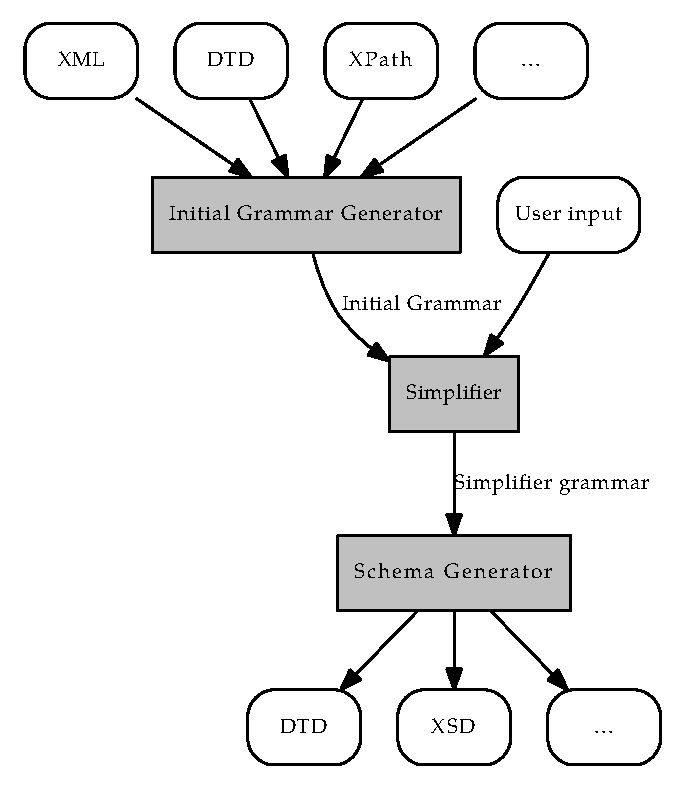
\includegraphics[width=\myscale\columnwidth]{inference_process}
	\caption{High-level view of the inference process} \label{inference_process}
\end{figure}
We divide the inference process into three steps (as illustrated in fig. \ref{inference_process}):
\begin{enumerate}
	\item Import of various formats (XML/XSD/DTD/XPath/\ldots) into an internal representation - \emph{Initial Grammar}.
	\item Simplification (generalization) of \emph{Initial Grammar} with optional help of user interaction.
	\item Export into various schema formats (XSD/DTD/\ldots).
\end{enumerate}	
Our internal representation is a regular grammar, i.e. a list of rules.
We represent the right side of grammar rule as a regular expression with our own set of classes to represent regexps.

On input, all various formats are at first converted into internal representation - from XML, rules are extracted as positive examples, concatenations; from XSD/DTD, rules are extracted as they are written in the schema. From XPath we extract only explicit concatenations for now.

Rules are sent to \jmodule{Simplifier} module, which has to do the simplification algorithm and return a \emph{Simplified Grammar}, which is then easily exported by \jmodule{Schema Generator} modules.

\begin{figure}
	\centering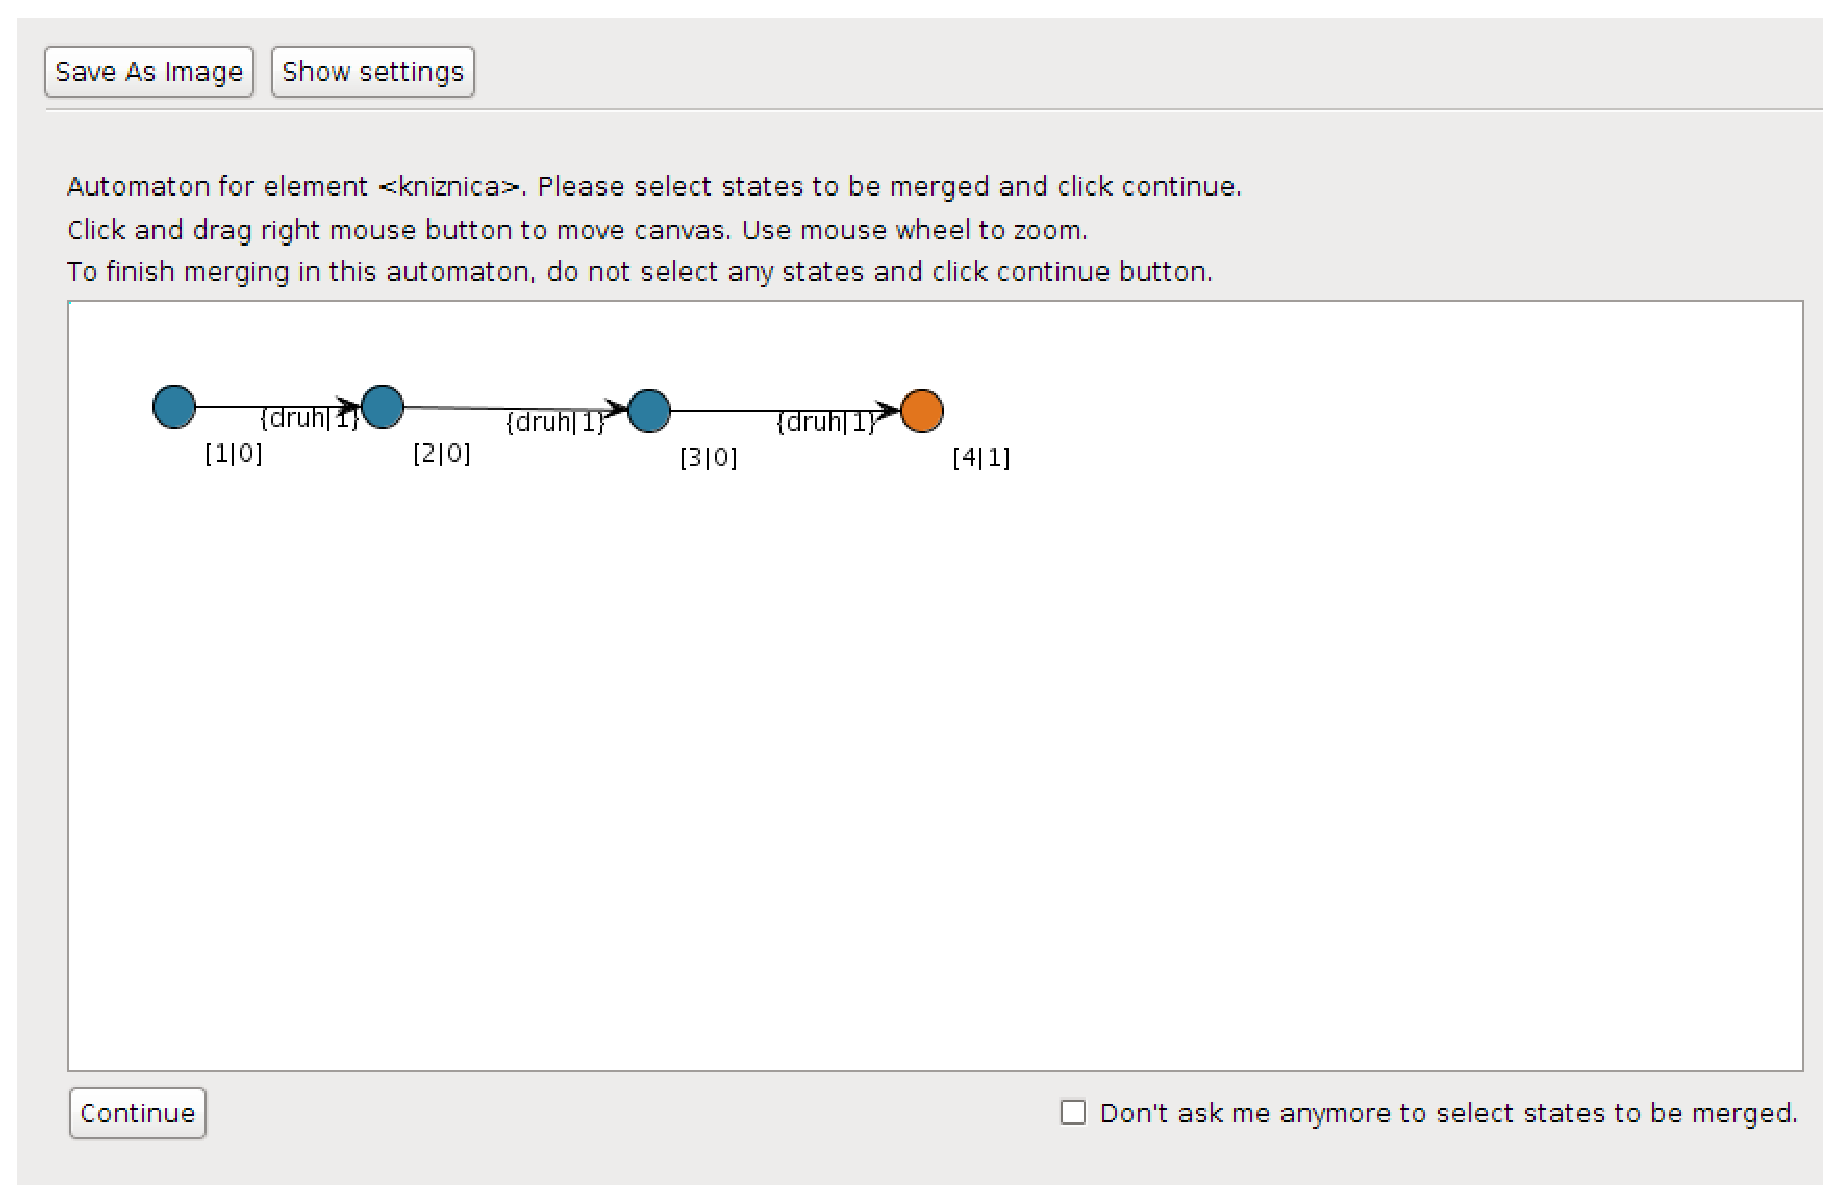
\includegraphics[width=\myscale\columnwidth]{screenshot}
	\caption{Visualization of automaton in inference process} \label{screenshot}
\end{figure}
Simplification can be either automatic, or user-aided.
We provide visualization of non-deterministic finite automata.
This helps algorithms that use merging state algorithms with user interaction.
Using simple API, algorithm developer can call our library to present the automaton to the user to make human decisions and continue in simplification process.
See figure \ref{screenshot} for an automaton visualization tool.

\begin{figure}
	\centering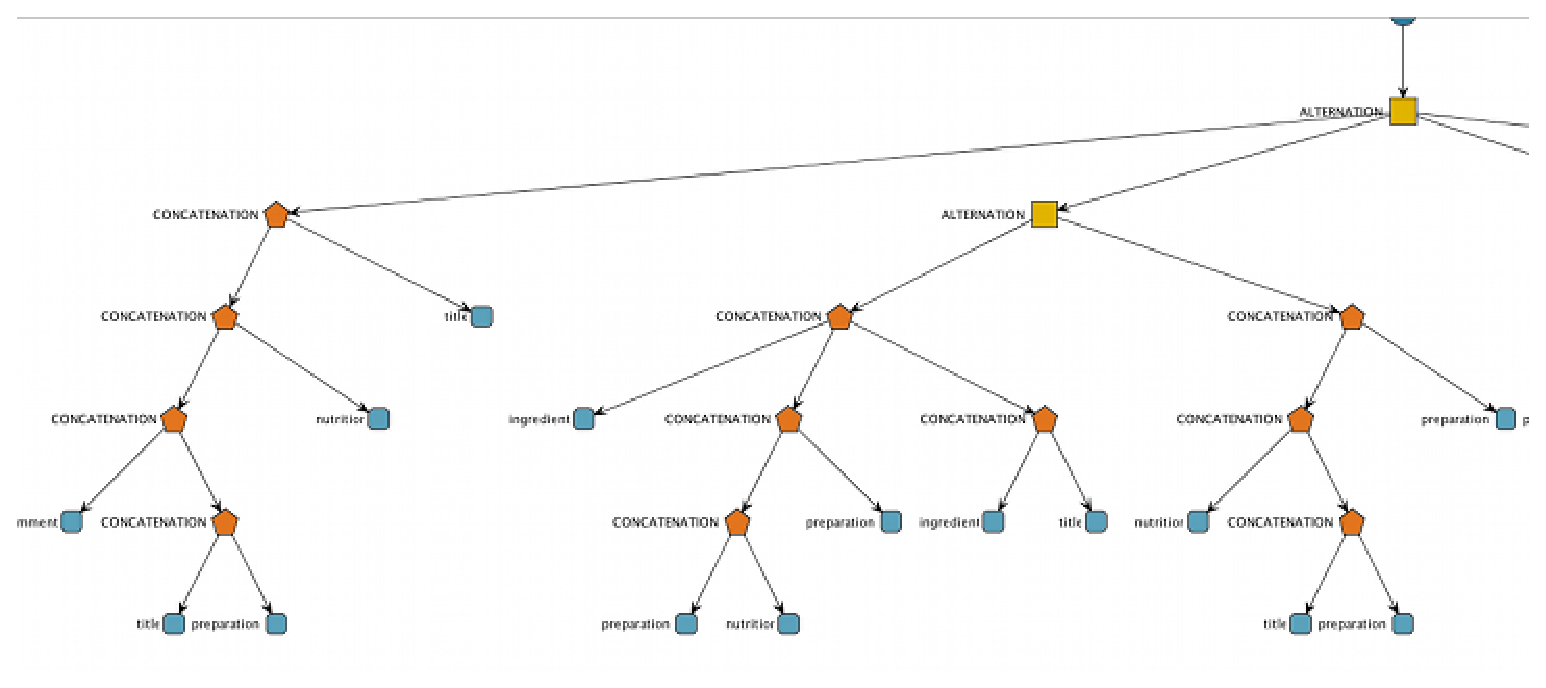
\includegraphics[width=\myscale\columnwidth]{ruledisplayer}
	\caption{Visualization of a grammar rule} \label{ruledisplayer}
\end{figure}
We provide visualization of rules themselves, which is useful for methods not using automata at all.
Algorithm can use API to display rules to user in progress (see fig. \ref{ruledisplayer}).

\section*{Extensibility}
Developers willing to experiment with their own algorithms need to take care only of \jmodule{Simplifier} module.
We provide a sample one, which is recursively divided into submodules.
One can find the exact place to replace functionality he wants, and replace only that part of the simplification chain.
It is still optional whether to use this new experimental module or the old, bundled one.
He doesn't need to code into jInfer sources, keeping his software installed in same NB instance as jInfer is enough. %TODO

As we implement \cite{ahonen}, good support for merging state algorithms is provided - automaton visualization for example.
We divide automaton state merging in two tasks: merging strategy and merging criterion.
Former one is responsible of deciding whether to merge two states or not.
It has to decide where to stop merging and work is done, it uses merging criterion to test two states equivalency and can measure automaton as it wants to decide whether to continue or stop process.
Merging criterion (we implement $k,h$-context) can be replaced and plugged into the merging strategy. One can implement for example $s,k$-strings (\cite{Garofalakis:2000:XSE:335191.335409}).

We provide replacable parts in automaton-to-regexp conversion problem, so one can replace our state removal method (with simple weighted heuristic).

Possibilities are open.

\section*{Open issues}
There are still many issues to be worked on.
First one is the set of supported input/output formats.
On input, one can imagine support for XML Queries, on output export to languages like Relax NG or Schematron. 
There is room for implementing schema visualization tool into jInfer, to enable user-aided schema refinement (to approach \cite{Bex:2008:SSI:1376616.1376750}).

For now we ignore content models of attribute and text node values, but there is an interface waiting to be implemented.
Thus, simple data type detection is waiting for its implementor.

Many algorithms published wait to be implemented as jInfer modules, perhaps some of them will be implemented in the course of our master theses.

\section*{Conclusion}
The framework presented in this paper aims to be the tool used to obtain schemas from XML/XSD/DTD files (and more after extension).
While maintaining a distributable bundle for users, with the best modules and algorithms implemented so far, we predict it will be used in future studies of new algorithms as a test environment.
Best of them will probably merged into jInfer source tree to aid common users to solve their schema inference problems quickly and easily.

Weak side of our solution is the lack of good quality automatic or semi-automatic algorithms to be used by common user, as well as the lack of content model inference.
Our goal was to produce a stable framework for future development and we hope to negate these issues by implementing our master theses in this environment, providing it with a bundle of different algorithms, solving different input and output formats and infering more concise schemas.

\nocite{*}
\newpage
\bibliographystyle{alpha}
\bibliography{literature}
\end{document}
